\chapter{Dynamic Model of the Quadrotor \label{ch:model}}

In this chapter, the derivation of the quadrotor model is provided. This result
is very important because it describes how the helicopter moves according to its
inputs. Thanks to these equations it is possible to define and predict the positions
reached by the helicopter by investigating just the four motor speeds. The model
equations will be ”inverted” in the next chapter (Control algorithms) to identify
which inputs are needed to reach a certain position.
\\\\
The first section (\fullref{sec:configurations}) shows the main idea of the quadrotor
dynamics and describes intuitively which movements are allowed and how it
manages to perform stationary flight (hovering).
\\\\
The second section () provides the model information
with physics and mathematical derivations. In this work, the Newton-Euler
formalism and the Euler angles theories have been chosen.
\\\\
In the third section (\fullref{sec:nonlinear}), additional information was added to
the model taking into account the whole motor system which is composed of the
motor itself, the reduction gears and the propeller.
\\\\
The last section (\fullref{sec:linearized}) provides an overview of the architecture:
connections between devices and abstraction of the software and task.

\section{Quadrotors Configurations}
\label{sec:configurations}
As the term `quadrotor' refers to a multirotor whose thrust is generated from four motors and propellers, quadrotors can be built in multiple ways as long as they comply with the established definition. There are some configurations that are already standardized being widely used by commercial manufacturers and hobbyists, such as the `+' and `X' configurations.
%\\\\
%\url{https://www.google.com/search?q=why+\%2B+or+x+configuration+quadcopter&ie=utf-8&oe=utf-8&client=firefox-b-ab&gfe_rd=cr&dcr=0&ei=Mr0BWrW9HtHk8AfXm7fADQ}
%\\\\
%\url{https://community.micro-motor-warehouse.com/t/vs-x-configuration/2673}
%\\\\
%\url{https://www.quora.com/Why-is-x-configuration-preferred-over-+-config-of-quadcopter}
%\\\\
%\url{https://www.rcgroups.com/forums/showthread.php?1203569-Quad-X-vs-configuration}


\subsection{`+' Configuration}
The geometry used in quadrotors built in `+' configuration is shown in Fig. \ref{fig:quadcopterplus}.
\\
\begin{figure}[H]
\begin{center}
  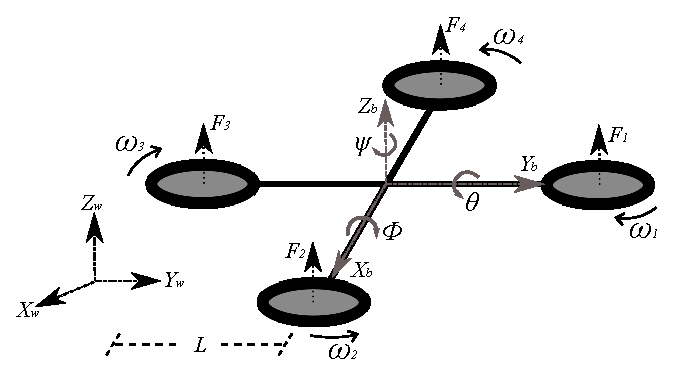
\includegraphics[width=0.90\textwidth]{quadcopterplus.eps}
\caption{Quadrotor geometry in `+' configuration} 
    \label{fig:quadcopterplus}
    \end{center}
\end{figure}
Where, ($\phi$, $\theta$, $\psi$) are the angular deviations (pitch, roll and yaw, respectively) of the quadrotor about the body-frame,
 ($x$, $y$, $z$) are the body-frame axes,  ($X_W$, $Y_W$, $Z_W$) are the earth-frame axes, $L$ is the distance from the quadrotor center of gravity ($CoG$) to the motors center, $F_{M_i}$ is the thrust force exerted by each motor $M_i$, and $\omega_i$ is the angular velocity of $M_i$, with $i = 1,2,3,4$. In this configuration, the body-frame axes $x$ and $y$, coincide with the lines that connect motors of opposite sides in the quadrotor frame.
\\\\
Although the quadrotor is a system with 6 degrees of freedom ($DoF$), the fact of having only four actuators, makes it an underactuated system. Therefore, it is only possible to reach a desired state for 4 degrees of freedom. However, it is possible to choose four control signals, or inputs, that represent the quadrotor basic movements and allow the quadrotor to achieve a desired position and attitude. This inputs are described below.
\begin{itemize}
\item \textbf{Throttle $T_u$ [$N$]}
The throttle $u$ is the total thrust force exerted parallel to the body-frame $z$-axis by the four motors. When the $\theta$ and $\phi$ angles are different from zero, the throttle generates accelerations, not only on the $Z_W$-axis, but also on the $X_W$ and $Y_W$ axes, as the body-frame $z$-axis and the $Z_W$ do not coincide.
\\\\
This control signal affects the speed of rotation of all motors, and therefore their thrust, in equal magnitude, and is set as
\begin{equation}
\label{ec:u+}
T_u = \sum_{i=1}^{4}F_{M_i}.
\end{equation}

\item \textbf{Yaw Torque $\tau_{\psi}$ [$N\cdot m$]}
As can be seen in Fig. \ref{fig:quadcopterplus}, $M_1$ and $M_3$ have a clockwise rotation while $M_2$ and $M_4$ rotate counter-clockwise. This configuration of opposite pairs rotational directions allows the system to control its conservation of momentum, and thus change its yaw angle in a controlled manner, just unbalancing the total momentum around the $z$-axis and without the need of a tail rotor used in the standard helicopter structure (\cite{Bresciani2008}). In `+' configuration, the fact that the pitch and roll angles are controlled using only two motors that rotate in the same direction, leads to large changes in the thrust force of the other two motors to achieve conservation of momentum.
\\\\
This conservation of momentum is controlled using the torque generated by each motor ($\tau_{M_i}$) around the body-frame $z$-axis, causing a turn in the direction opposite to the rotation of the motor. Taking into account that the torque $\tau_\psi$ is positive when it generates a clock-wise rotation around the $z$-axis, only $M_2$ and $M_4$ contribute positively to it, while the others have a negative contribution to $\tau_\psi$. Thus, the total torque around the $z$-axis is set as
\begin{equation}
\label{ec:taupsiTM}
\tau_{\psi} = \tau_{M_2} + \tau_{M_4} - \tau_{M_1} - \tau_{M_3}.
\end{equation}
Each torque $\tau_{M_i}$ has a linear relationship with the thrust applied by the motor, with $K_M$ being the proportional constant and
\begin{equation}
\label{ec:taumi}
\tau_{M_{i}} = K_{M}F_{M_i}.
\end{equation}
Replacing (\ref{ec:taumi}) in (\ref{ec:taupsiTM}) the total torque $\tau_\psi$ dependence on the forces $F_{M_i}$ is got as
\begin{equation}
\label{ec:taupsi+}
\tau_{\psi} = K_{m}(F_{M_2} + F_{M_4} - F_{M_1} - F_{M_3}).
\end{equation}

\item \textbf{Roll Torque $\tau_{\theta}$ [$N\cdot m$]}
The roll torque $\tau_\theta$ is the torque exerted on the $x$-axis and about the $y$-axis. In the `+' configuration, the only motors that affect the quadrotor rotation with respect to the $x$-axis are $M_2$ and $M_4$. These in turn do not affect the rotation with respect to the $y$-axis. In this case, the torques are generated by the forces $F_{M_2}$ and $F_{M_4}$ being applied at a distance $L$ from the quadrotor $CoG$. Considering a positive $\tau_\theta$ as the one causing a counter clock-wise rotation about the $y$-axis, the roll torque in `+' is set as
\begin{equation}
\label{ec:tautheta+}
\tau_{\theta} = L(F_{M_4}-F_{M_2}).
\end{equation}

\item \textbf{Pitch Torque $\tau_{\phi}$ [$N\cdot m$]}
Unlike the roll torque, the pitch torque $\tau_\phi$ is the one exerted on the $y$-axis about the $x$-axis. As exposed in Fig. \ref{fig:quadcopterplus}, $M_1$ and $M_3$ are the motors applying the forces that create this torque. Being $\tau_\phi$ positive when clock-wise rotation about the $x$-axis is caused, it is defined for a `+' configuration as
\begin{equation}
\label{ec:tauphi+}
\tau_{\phi} = L(F_{M_3}-F_{M_1}).
\end{equation}
\end{itemize}

\subsubsection{Inputs Setting in `+' Configuration}
Summarizing the description of the four inputs in the quadrotor represented in a `+' configuration, these are established as linear combinations of the motors forces $F_{M_i}$ and can be represented as a system of linear equations in matrix representation based on equations (\ref{ec:u+}), (\ref{ec:taupsi+}), (\ref{ec:tautheta+}) and (\ref{ec:tauphi+}). Thus, the vector of inputs $U_{(+)}$ is defined as
\begin{equation}
	U_{(+)} = \begin{bmatrix}
	T_u\\[5pt]
	\tau_{\psi}\\[5pt]
	\tau_{\theta}\\[5pt]
	\tau_{\phi}
	\end{bmatrix} = \begin{bmatrix}
	1 & 1 & 1 & 1 \\[5pt]
	-K_{m} & K_{m} & -K_{m} & K_{m}\\[5pt]
	0 & -L & 0 & L\\[5pt]
	-L & 0 & L & 0
							\end{bmatrix}
\begin{bmatrix}
F_{M_1}\\[5pt]
F_{M_2}\\[5pt]
F_{M_3}\\[5pt]
F_{M_4}
\end{bmatrix}.
	\label{ec:U_+}						
\end{equation}

\subsection{`X' Configuration}
Following the same nomenclature used in the `+' configuration, in `X' configuration, the quadrotor frame is rotated $\pi/4\ rad$ about the $z$-axis in the body-frame, as shown in Fig. \ref{fig:quadrotorX}. 
\\\\
In this case, the front-line in the quadrotor is set between $M_1$ and $M_4$, while $M_2$ and $M_3$ define its back line. Using the `X' configuration, the roll and pitch torques are applied using the forces exerted by all the motors at a distance $L_X = L\cdot \cos(\pi/4)$.  The geometry used in this configuration is shown in Fig. \ref{fig:quadrotorX}.
\begin{figure}[H]
\begin{center}
  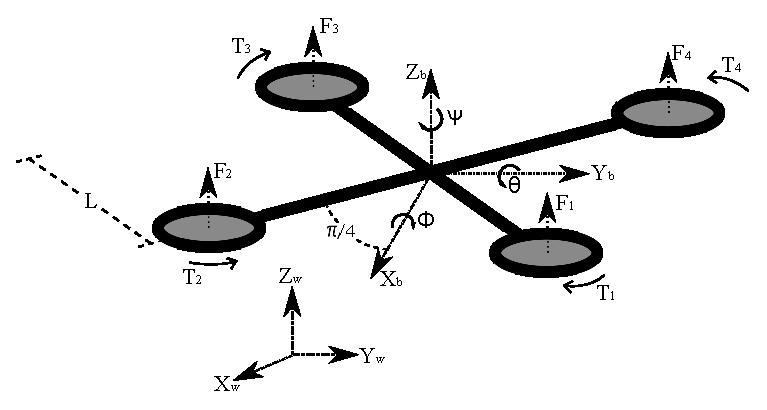
\includegraphics[width=0.97\textwidth]{quadcopter1.eps}
% figure caption is below the figure
\caption{Quadrotor geometry in `X' configuration} 
    \label{fig:quadrotorX}
    \end{center}
\end{figure}
The quadrotor inputs in `X' configuration do not change with respect to the + configuration, but it does change the way $\tau_\theta$ and $\tau_\phi$ are defined with respect to the forces $F_{M_i}$. The inputs description for the quadrotor `X' configuration is defined as follows.
\begin{itemize}
\item \textbf{Throttle $T_u$ [$N$]}\\\\
The total thrust exerted by the four motors in the quadrotor is not changed between the `+' and `X' configurations. Hence, the throttle $u$ is defined in the same way as in `+' configuration as
\begin{equation}
\label{ec:ux}
T_u = \sum_{i=1}^{4}F_{M_i}.
\end{equation}

\item \textbf{Yaw Torque $\tau_{\psi}$ [$N\cdot m$]}\\\\
As the $z$-axis is not modified between the `+' and `X' configurations, and the motors rotate in the same direction as in the other configuration, the yaw torque $\tau_\psi$ is set as
\begin{equation}
\label{ec:taupsix}
\tau_{\psi} = K_{m}(F_{M_2} + F_{M_4} - F_{M_1} - F_{M_3}).
\end{equation}

\item \textbf{Roll Torque $\tau_{\theta}$ [$N\cdot m$]}\\\\
In `X' configuration, $L_{X} = L\cdot \cos\left(\pi/4\right)$ is the real distance between the point of application of the roll and pitch torques and the quadrotor center of mass along the $x$ and $y$ axes (\cite{Faessler2016}). Also, as shown in Fig. \ref{fig:quadrotorX}, each of the four motors affects these torques. For the roll torque $\tau_{\theta}$, rhe motors $M_3$ and $M_4$ contribute positively to $\tau_\theta$, while $M_1$ and $M_2$ have a negative contribution to this torque. Then, for the `X' configuration, the roll torque is set as
\begin{equation}
\label{ec:tauthetax}
\tau_{\theta} = L_{X}(F_{M_3}+F_{M_4}-F_{M_2}-F_{M_1}).
\end{equation}

\item \textbf{Pitch Torque $\tau_{\phi}$ [$N\cdot m$]}\\\\
As in the roll torque, the pitch torque $\tau_{\phi}$ is affected by the forces exerted by the four motors in the quadrotor in `X' configuration. Due to the clock-wise positive direction of the $\phi$ angle, and keeping $L_X$ as the distance between the quadrotor $CoG$ and the point of application of the force on each axis, the pitch torque for the `X' configuration is defined as
\begin{equation}
\label{ec:tauphix}
\tau_{\phi} = L_{X}(F_{M_2}+F_{M_3}-F_{M_1}-F_{M_4}).
\end{equation}

\end{itemize}





\subsubsection{Inputs Setting in `X' Configuration}
In the `X' configuration, the quadrotor inputs remain the same with respect to the `+' configuration. However the torques $\tau_\theta$ and $\tau_\phi$ are affected by the interaction of all the motors and the change in the distance of the point of application of the forces $F_{M_i}$ on the $x$ and $y$ axes. The system of linear equations that shows the inputs setting for a quadrotor in `X' configuration is based on equations (\ref{ec:ux}), (\ref{ec:taupsix}), (\ref{ec:tauthetax}) and (\ref{ec:tauphix}), and is defined as
\begin{equation}
	U_{(X)} = \begin{bmatrix}
	T_u\\[5pt]
	\tau_{\psi}\\[5pt]
	\tau_{\theta}\\[5pt]
	\tau_{\phi}
	\end{bmatrix} = \begin{bmatrix}
	1 & 1 & 1 & 1 \\[5pt]
	-K_{m} & K_{m} & -K_{m} & K_{m}\\[5pt]
	-L_{X} & -L_{X} & L_{X} & L_{X}\\[5pt]
	-L_{X} & L_{X} & L_{X} & -L_{X}
							\end{bmatrix}
\begin{bmatrix}
F_{M_1}\\[5pt]
F_{M_2}\\[5pt]
F_{M_3}\\[5pt]
F_{M_4}
\end{bmatrix}.
	\label{ec:U_X}						
\end{equation}

\subsubsection{Maximum Torque About $x$ and $y$ axes in `X' Configuration}
In `+' configuration, the torques around the $x$ and $y$ axes are set using just two motors applying a force at a distance $L$ from the quadrotor $CoG$. This implies that, for example in the case of roll torque $\tau_\theta$, the maximum torque $\tau_{\theta max (+)}$ is achieved when $F_{M_4} = F_{M_i max}$ and $F_{M_3} = 0$, where $F_{M_i max}$ is the maximum thrust of the motors. Then, in `+' configuration, the $\tau_{\theta max (+)}$ is set as
\begin{equation}
\tau_{\theta max (+)} = L\cdot F_{M_i max}
\end{equation}
On the other hand, the torques around the $x$ and $y$ axes in `X' configuration depend on the forces of the four motors in the quadrotor, which are applied at a distance $L_{X} = L\cdot \cos(\pi/4)$ from the quadrotor $CoG$. Continuing with the example of the roll torque, in `X' configuration the maximum torque $\tau_{\theta max (X)}$ is achieved when $F_{M_3} = F_{M_4} = F_{M_i max}$ and $F_{M_1} = F_{M_2} = 0$. Hence, the maximum torque about the $y$-axis in `X' configuration is
\begin{align}
\begin{split}
\tau_{\theta max (X)} & = L\cdot \cos(\pi/4) \cdot 2 \cdot F_{M_i max}\\[5px]
\tau_{\theta max (X)} & = 2\cdot \cos(\pi/4) \cdot \tau_{\theta max (+)}\\[5px]
\end{split}
\end{align}
Thereby, the quadrotor in `X' configuration has $2\cdot \cos(\pi/4)$ times more available torque to rotate about the $x$ and $y$ axes, when compared with the `+' configuration, and therefore it can achieve $41.42\ \%$ more rotational acceleration about the $x$ and $y$ axes.


\section{Nonlinear Model}
\label{sec:nonlinear}

This section describes the dynamic modeling used to perform the quadrotor control, based on the study carried out in \cite{Bresciani2008} and \cite{Bouabdallah2007}. This model represents the quadrotor as a solid symmetrical object subject to a total thrust ($u$) and three torques ($\tau_\psi$, $\tau_\theta$ and $\tau_\phi$), without considering the dynamics of the actuators. The modeling of the quadrotor system is done by two different methods. The Newton-Euler approach is based on the quadrotor body-frame, while the Euler-Lagrange approach bases its translational equations in the earth-frame while keeping its rotational equations related to the body-frame.

\subsection{Newton-Euler Approach}
Following the quadrotor geometry shown in Fig. \ref{fig:quadrotorX}, the quadrotor position vector ($\mathbf{\Xi}$), composed by the translational position ($\mathbf{\Gamma_W}$ [$m$]) and rotational position ($\mathbf{\Theta_W}$ [$rad$]) with respect to the earth-frame, is defined as
\begin{equation}
\mathbf{\Xi} = \begin{bmatrix}
\mathbf{\Gamma_W} \\ \mathbf{\Theta_W}
\end{bmatrix} = \begin{bmatrix}
x \\ y \\ z \\ \psi \\ \theta \\ \phi
\end{bmatrix}.
\end{equation}
On the other hand, the quadrotor velocity vector ($\mathbf{\nu}$) is composed by the translational ($\mathbf{V_B}$ [$m\cdot s^{-1}$]) and rotational ($\mathbf{\Omega_B}$ [$rad\cdot s^{-1}$]) velocities with respect to the body-frame as
\begin{equation}
\mathbf{\nu} = \begin{bmatrix}
\mathbf{V_B} \\ \mathbf{\Omega_B}
\end{bmatrix} =
\begin{bmatrix}
u \\ v \\ w \\ p \\ q \\ r
\end{bmatrix}.
\end{equation}
There exists a generalized matrix
\begin{equation}
\mathbf{J_\Theta} = \begin{bmatrix}
\mathbf{R_{b}^{w}} & \mathbf{0_{3\times 3}} \\
\mathbf{0_{3\times 3}} & \mathbf{T_{b}^{w}}
\end{bmatrix},
\end{equation}
that ensures that
\begin{equation}
\mathbf{\dot{\Xi}} = \mathbf{J_\Theta}\mathbf{\nu},
\end{equation}
where $\mathbf{0_{3\times 3}}$ is a $3\times 3$-matrix filled with zeros, $\mathbf{R_{b}^{w}}$ is the rotation matrix and $\mathbf{T_{b}^{w}}$ the transfer matrix, defined as
\begin{equation}
\mathbf{R_{b}^{w}} = \begin{bmatrix}
c_\theta c_\psi & c_\psi s_\theta s_\phi-c_\phi s_\psi & s_\phi s_\psi+c_\phi c_\psi s_\theta\\
c_\theta s_\psi & s_\psi s_\theta s_\phi+c_\phi c_\psi & c_\phi s_\psi s_\theta - s_\phi c_\psi\\
-s_\theta & c_\theta s_\phi & c_\theta c_\phi
\end{bmatrix},
\end{equation}
\begin{equation}
\mathbf{T_{b}^{w}} = \begin{bmatrix}
1 & s_\phi t_\theta & c_\phi t_\theta\\
0 & c_\phi & -s_\phi\\
0 & s_\phi / c_\theta & c_\phi / c_\theta 
\end{bmatrix},
\end{equation}
with $s_\theta = \sin(\theta)$, $c_\theta = \cos(\theta)$, and $t_\theta = \tan(\theta)$.
\\\\
As the quadrotor is assumed to be a rigid body of 6 $DoF$, its dynamics consider the mass ($m$ [$kg$]) and the inertia matrix ($\mathbf{J}$ [$kg\cdot m^{2}$]) of it, and are described as
\begin{equation}
\label{eqn:eomNewtonEuler}
\begin{bmatrix}
m\mathbf{I_{3\times3}} & \mathbf{0_{3\times 3}} \\
\mathbf{0_{3\times 3}} & \mathbf{J}
\end{bmatrix}
\begin{bmatrix}
\mathbf{\dot{V}_{B}} \\ \mathbf{\dot{\Omega}_B}
\end{bmatrix}
+ \begin{bmatrix}
\mathbf{\Omega_B} \times m\mathbf{V_{B}} \\
\mathbf{\Omega_B} \times \mathbf{J}\mathbf{\Omega_B}
\end{bmatrix}
=
\begin{bmatrix}
\mathbf{F_{B}} \\ \mathbf{\tau_{B}}
\end{bmatrix},
\end{equation}
where $\mathbf{I}$ is the identity matrix, $\mathbf{\dot{V}_{B}}$ is the quadrotor translational acceleration in the body-frame, $\mathbf{\dot{\Omega}_B}$ is the quadrotor angular acceleration in the body-frame, $\mathbf{F_{B}}$ is the quadrotor force vector and $\mathbf{\tau_{B}}$ is the quadrotor torques vector. 
\begin{figure}[h]
\begin{center}
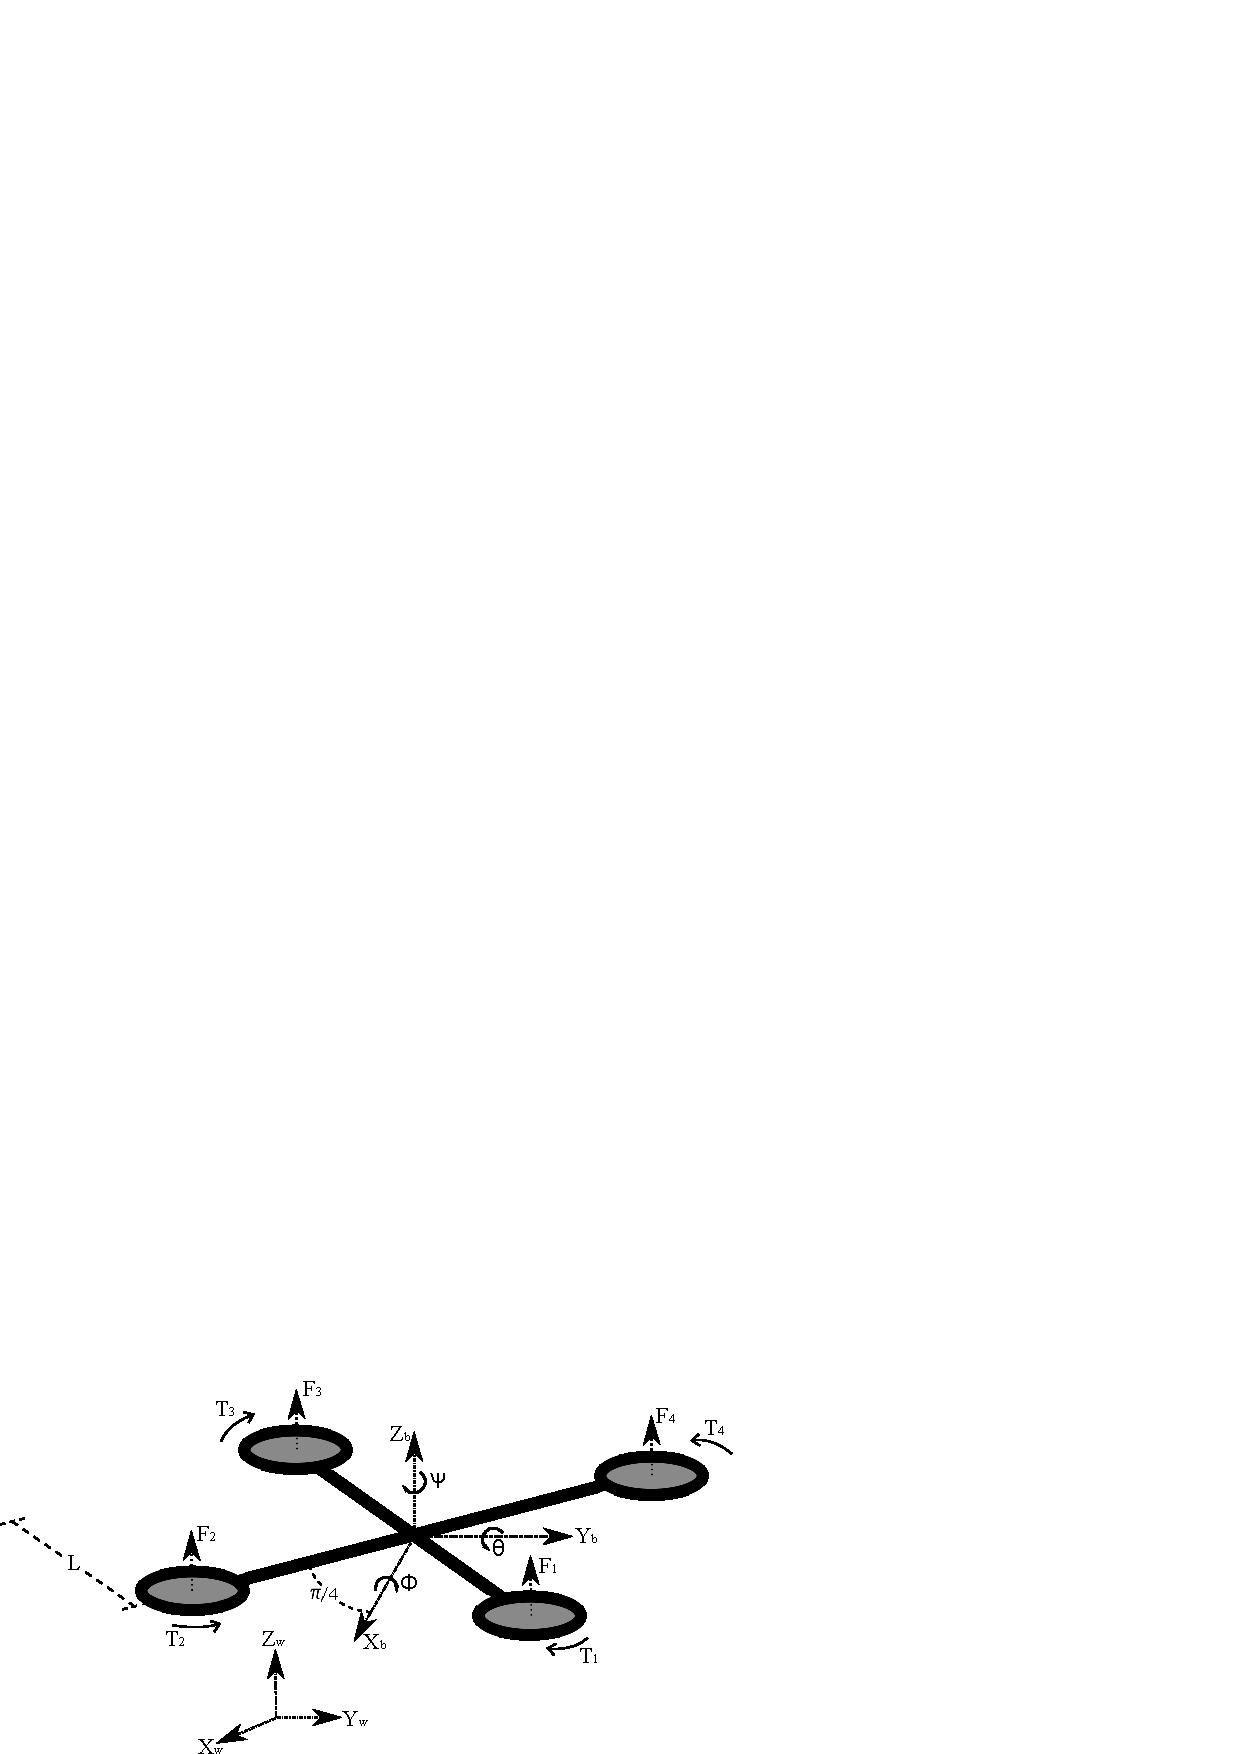
\includegraphics[width=6.8cm]{quadcopter1.pdf}    
\caption{Quadrotor squeme with movement axis and thrust forces.} 
\label{fig:quadfigure}
\end{center}
\end{figure}
\\From this Newton-Euler approach, the quadrotor equations obtained for the translational and angular accelerations are
\begin{align}\label{eqn:eom}
\begin{split}
\ddot{x} &= \frac{u_{1}}{m}(\cos(\phi)\sin(\theta)\cos(\psi) + \sin(\phi)\sin(\psi)), \\
\ddot{y} &= \frac{u_{1}}{m}(\cos(\phi)\sin(\theta)\sin(\psi) - \sin(\phi)\cos(\psi)), \\
\ddot{z} &= \frac{u_{1}}{m}(\cos(\phi)\cos(\theta)) - g, \\
\ddot{\psi} &= \dot{\phi}\dot{\theta}\dfrac{J_{xx}-J_{yy}}{J_{zz}} + \dfrac{u_{2}}{J_{zz}},\\
\ddot{\theta} &= \dot{\phi}\dot{\psi}\dfrac{J_{zz}-J_{xx}}{J_{yy}} + \dfrac{u_{3}}{J_{yy}}, \\
\ddot{\phi} &= \dot{\theta}\dot{\psi}\dfrac{J_{yy}-J_{zz}}{J_{xx}} +  \dfrac{u_{4}}{J_{xx}},
\end{split}
\end{align}
with
\begin{align}
\label{eqn:eom1}
\begin{split}
u_{1} &= u-mg = F_{1} + F_{2} + F_{3} + F_{4}, \\
u_{2} &= \tau_{\psi} = T_{2} + T_{4} - T_{1} - T_{3}, \\
u_{3} &= \tau_{\theta} = L(F_{4} + F_{1} - F_{2} - F_{3}), \\
u_{4} &= \tau_{\phi} = L(F_{1} + F_{2} - F_{3} - F_{4}),
\end{split}
\end{align}
where $u$ is the total throttle applied by the motors, $\tau_{\phi}$, $\tau_{\theta}$, $\tau_{\psi}$ the rolling, pitching and yawing moment, $J_{xx}$, $J_{yy}$ and $J_{zz}$ are the moments of inertia around the $x$, $y$ and $z$ axis respectively, while $L$ is the distance from any motor to the center of mass of the quadrotor and $F_{i}$ and $T_{i}$, with $i$ $\in$ ${1,2,3,4}$, are the thrust force and torque exerted from each motor. The non-linear model of the quadrotor is linearized using the Jacobian of the non-linear model around an equilibrium point where $V_{B}$, $\omega_{B}$, $\psi$, $\theta$ and $\phi$ tend to zero, as
\begin{align}
\label{eqn:linear}
\begin{split}
\ddot{x} &= -g\theta, \\
\ddot{y} &= g\phi,  \\
\ddot{z} &= u_{1}/m, \\
\ddot{\psi} &= u_{2}/I_{zz}, \\
\ddot{\theta} &= u_{3}/I_{yy}, \\
\ddot{\phi} &= u_{4}/I_{xx}, 
\end{split}
\end{align}
and can be defined as a state space representation following the system
\begin{equation}\label{eqn:ss}
G = \mleft[
\begin{array}{c|c}
  A & B \\
  \hline
  C & D
\end{array}
\mright]
\end{equation}
where $A$ is the system matrix, $B$ is the input matrix, $C$ is the output matrix and $D$ is the feedthrough matrix. The state vector $X$, input vector $U$, and outputs vector $Y$ are
\setcounter{MaxMatrixCols}{20}
\begin{equation}
X = \begin{bmatrix}
x & y & z & \dot{x} & \dot{y} & \dot{z} & \psi & \theta & \phi & \dot{\psi} & \dot{\theta} & \dot{\phi} 
\end{bmatrix}^{T},
\end{equation}
\begin{equation}
U = \begin{bmatrix}
u_{1} & u_{2} & u_{3} & u_{4}
\end{bmatrix}^{T},
\end{equation}
\begin{equation}
Y = \begin{bmatrix}
x & y & z & \psi
\end{bmatrix}^{T}.
\end{equation}


\subsection{Euler-Lagrange Approach}
The general coordinates representing the position and attitude of the quadrotor are defined as
\begin{equation}
	\Xi=\begin{bmatrix}
	\xi & \eta
	\end{bmatrix}^{T},
	\label{ec:coorgenerales}
\end{equation}
where $\xi=\begin{bmatrix}
x & y & z
\end{bmatrix}^{T}$ is the vector representing the position of the center of mass of the quadrotor relative to the body reference frame shown in Fig. \ref{fig:marcoreferencia} and $\eta=\begin{bmatrix}
\psi & \theta & \phi
\end{bmatrix}^{T}$ represent the quadrotor attitude.
\\\\
The Lagrangian of the quadrotor is defined by
\begin{equation}
	L(\Xi,\dot{\Xi})=K_{trans}+K_{rot} - U,	
	\label{ec:lagrangiano}
\end{equation}
where $ K_{trans} = \dfrac{m}{2}\dot{\xi}^{T}\dot{\xi} $ is the translational kinetic energy, $ K_{rot} = \dfrac{1}{2}\dot{\eta}^{T}J\dot{\eta} $ is the rotational kinetic energy, $ U=mgz $ is the potential energy, $m$ is the quadrotor mass , $z$ is the quadrotor elevation, $g$ is the gravity acceleration magnitude, and $J$ is the inertial matrix. The dynamic model of the quadrotor is derived from the Euler-Lagrange equation
\begin{equation}
	\dfrac{d}{dt}\dfrac{\partial L}{\partial \dot{\Xi}}-\dfrac{\partial L}{\partial \Xi}=
	\begin{bmatrix}
	F_{\xi}\\
	\tau
	\end{bmatrix},
	\label{ec:eulerlag}
 \end{equation} 
where $F_{\xi}=R_{b}^{w}\hat{F_{b}}$ is the translational force applied to the quadrotor by the four motors, $\tau$ contains the rolling, pitching and yawing torques ($\tau_\theta$, $\tau_\phi$, $\tau_\psi$).
\\\\
In the quadrotor body-frame, the translational force $\hat{F_{b}}$ is only applied in the $z_{b}$ axis as shown in Fig. \ref{fig:marcoreferencia}. This force is represented by
\begin{equation}
	\hat{F_{b}}=\begin{pmatrix}
	0\\
	0\\
	u
	\end{pmatrix} = \begin{pmatrix}
	0\\
	0\\
	\sum_{i=1}^{4}F_{M_i}
	\end{pmatrix}  ,
 \label{ec:fuerzas}
 \end{equation} 
with $ F_{M_i} $ being the force, in N, exerted by the motor $ M_{i}$, as shown in Fig. \ref{fig:marcoreferencia}.
\\\\
The force $ F_{M_i} $ has a linear dependency with the square of the motor angular velocity, defined as
\begin{equation}
	F_{M_i}=k_{i}w_{i}^{2},
	\label{ec:fi}
\end{equation}
where $ w_{i} $ is the angular velocity of the motor, and $ k_{i} $ is a proportional constant. However, in practice $F_{M_i}$ must be set using the PWM signal input of an ESC. The thrust-PWM relation is found experimentally and is shown in Section \ref{sec:Implementation}.
\\\\
The Euler-Lagrange equations can be divided in two parts, one for the $\xi$ coordinates and another for the $\eta$ coordinates, getting
\begin{equation}
\label{eqn:E-L1}
\ddot{\xi} =
\begin{bmatrix}
\ddot{x} \\ \ddot{y} \\ \ddot{z}
\end{bmatrix} 
=
\begin{bmatrix}
\frac{u_{1}}{m}(C_\phi S_\theta C_\psi + S_\phi S_\psi) \\
 \frac{u_{1}}{m}(C_\phi S_\theta S_\psi - S_\phi C_\psi) \\
\frac{u_{1}}{m}(C_\phi C_\theta) - g
\end{bmatrix},
\end{equation}
\begin{equation}
\label{eqn:E-L2}
\ddot{\eta} =
\begin{bmatrix}
\ddot{\psi} \\ \ddot{\theta} \\ \ddot{\phi}
\end{bmatrix} 
 =
\begin{bmatrix}
\dot{\phi}\dot{\theta}\dfrac{J_{xx}-J_{yy}}{J_{zz}} + \dfrac{u_{2}}{J_{zz}} \\
\dot{\phi}\dot{\psi}\dfrac{J_{zz}-J_{xx}}{J_{yy}} + \dfrac{u_{3}}{J_{yy}} \\
 \dot{\theta}\dot{\psi}\dfrac{J_{yy}-J_{zz}}{J_{xx}} +  \dfrac{u_{4}}{J_{xx}}
\end{bmatrix},
\end{equation}
where, $\begin{bmatrix}
u_{1},\ u_{2},\ u_{3}, \ u_{4}
\end{bmatrix}^{T} = \begin{bmatrix}
u,\ \tau_{\psi},\ \tau_{\theta},\ \tau_{\phi}
\end{bmatrix}^{T} $, and $ (J_{xx}, J_{yy}, J_{zz}) $ are the moments of inertia around the quadrotor body-frame axes \cite{Emam2016, Badr2016}.
\\\\

that is a simplified representation of the quadrotor complete model found in \cite{Bouabdallah2007}.

\section{Linearized Model}
\label{sec:linearized}
\setcounter{MaxMatrixCols}{20}
\subsection{Jacobian Linearization}
\cite{Sabatino2015}
\\\\
The Euler-Lagrange equations in (\ref{eqn:E-L1}) and (\ref{eqn:E-L2}) are linearized using their Jacobian around the hover state where $\begin{bmatrix}
\eta,\ \dot{\eta},\ \dot{\xi}
\end{bmatrix} \to \begin{bmatrix}
0,\ 0,\ 0
\end{bmatrix}$, getting
\begin{equation}
\label{eqn:linear}
\ddot{q}
=
\begin{bmatrix}
g\theta \\
g\phi\\
u_{1}/m \\
u_{2}/J_{zz} \\
u_{3}/J_{yy} \\
u_{4}/J_{xx}
\end{bmatrix},
\end{equation}

As said above, in order to perform the linearization, an equilibrium point is
needed. Such an equilibrium point can be:
\begin{equation}
\overline{\mathbf{x}} = \begin{bmatrix}
\overline{x} & \overline{y} & \overline{z} & 0 & 0 & 0 & 0 & 0 & 0 & 0 & 0 & 0
\end{bmatrix}^{T}
\end{equation}
From the equations, we can find that the equilibrium point (2.29) is obtained by
the constant input value:
\begin{equation}
\overline{\mathbf{u}} = \begin{bmatrix}
mg & 0 & 0 & 0
\end{bmatrix}^{T}
\end{equation}
with $mg$ being the lift force.
\\\\
The linearized model of the quad-rotor helicopter written as a state space model is given by

\begin{align*}
\dot{\mathbf{x}}(t) = & A\mathbf{x}(t)+B\mathbf{u}(t),\\
\mathbf{y}(t) = & C\mathbf{x}(t),
\end{align*}
where
\begin{align}
\begin{split}
A  = \frac{\partial f(\mathbf{x},\mathbf{u})}{\partial \mathbf{x}}\Bigr|_{\substack{\mathbf{x}=\overline{\mathbf{x}}\\\mathbf{u}=\overline{\mathbf{u}}}} = & 
\begin{bmatrix}
0 & 1 & 0 & 0 & 0 & 0 & 0 & 0 & 0 & 0 & 0 & 0\\[2px]
0 & 0 & 0 & 0 & 0 & 0 & 0 & 0 & g & 0 & 0 & 0\\[2px]
0 & 0 & 0 & 1 & 0 & 0 & 0 & 0 & 0 & 0 & 0 & 0\\[2px]
0 & 0 & 0 & 0 & 0 & 0 & 0 & 0 & 0 & 0 & g & 0\\[2px]
0 & 0 & 0 & 0 & 0 & 1 & 0 & 0 & 0 & 0 & 0 & 0\\[2px]
0 & 0 & 0 & 0 & 0 & 0 & 0 & 0 & 0 & 0 & 0 & 0\\[2px]
0 & 0 & 0 & 0 & 0 & 0 & 0 & 1 & 0 & 0 & 0 & 0\\[2px]
0 & 0 & 0 & 0 & 0 & 0 & 0 & 0 & 0 & 0 & 0 & 0\\[2px]
0 & 0 & 0 & 0 & 0 & 0 & 0 & 0 & 0 & 1 & 0 & 0\\[2px]
0 & 0 & 0 & 0 & 0 & 0 & 0 & 0 & 0 & 0 & 0 & 0\\[2px]
0 & 0 & 0 & 0 & 0 & 0 & 0 & 0 & 0 & 0 & 0 & 1\\[2px]
0 & 0 & 0 & 0 & 0 & 0 & 0 & 0 & 0 & 0 & 0 & 0
\end{bmatrix}, \\[15px]
B = \frac{\partial f(\mathbf{x},\mathbf{u})}{\partial \mathbf{u}}\Bigr|_{\substack{\mathbf{x}=\overline{\mathbf{x}}\\\mathbf{u}=\overline{\mathbf{u}}}} = & 
\begin{bmatrix}
0 & 0 & 0 & 0 & 0 & \frac{1}{m} & 0 & 0 & 0 & 0 & 0 & 0\\[5px]
0 & 0 & 0 & 0 & 0 & 0 & 0 & \frac{1}{I_{zz}} & 0 & 0 & 0 & 0\\[5px]
0 & 0 & 0 & 0 & 0 & 0 & 0 & 0 & 0 & \frac{1}{I_{yy}} & 0 & 0\\[5px]
0 & 0 & 0 & 0 & 0 & 0 & 0 & 0 & 0 & 0 & 0 & \frac{1}{I_{xx}}
\end{bmatrix}^{T},\\[15px]
C = &
\begin{bmatrix}
1 & 0 & 0 & 0 & 0 & 0 & 0 & 0 & 0 & 0 & 0 & 0\\
0 & 0 & 1 & 0 & 0 & 0 & 0 & 0 & 0 & 0 & 0 & 0\\
0 & 0 & 0 & 0 & 1 & 0 & 0 & 0 & 0 & 0 & 0 & 0\\
0 & 0 & 0 & 0 & 0 & 0 & 1 & 0 & 0 & 0 & 0 & 0 
\end{bmatrix},
\end{split}
\end{align}

with the parameters  

$m=0.64 $ kg, 

$g=9.81$ m/s.


The state vector is defined as

\begin{align*}
x(t)=&
\begin{bmatrix}
r_x & \dot{r}_x & r_y & \dot{r}_y & r &\dot{r}_z 
\end{bmatrix}^T,
\end{align*}
and the control inputs as
\begin{align*}
u(t)=&
\begin{bmatrix}
u_1 & u_2 &u_3 & u_4
\end{bmatrix}^T,
\end{align*}

and the output vector is defined as

\begin{align*}
r(t)=
\begin{bmatrix}
r_{x} & r_{y} & r_{z}
\end{bmatrix}^T.
\end{align*}

\subsection{Thrust Compensation}
\url{https://robotics.stackexchange.com/questions/4247/tilt-compensated-motor-output-to-keep-altitude-for-quadcopter}
Recalling the rotation matrix $R_{b}^{w}$,
\begin{equation}
R_{b}^{w} = \begin{bmatrix}
c\theta c\psi & c\psi s\theta s\phi-c\phi s\psi & s\phi s\psi+c\phi c\psi s\theta\\
c\theta s\psi & s\psi s\theta s\phi+c\phi c\psi & c\phi s\psi s\theta - s\phi c\psi\\
-s\theta & c\theta s\phi & c\theta c\phi
\end{bmatrix}
\end{equation}
\begin{equation}
u = u^{*} \cos{\theta}\cos{\phi}
\end{equation}
\begin{equation}
u^{*} = \dfrac{u}{\cos{\theta}\cos{\phi}}
\end{equation}
\section{Conclusions}
This chapter presented the design of the two vehicles developed in this thesis.
The test-bench and the OS4. The first system is only capable of 3 DoF which
facilitates the testing of the controllers. However, it is possible to detach the
flying part in order to test free flights. Before designing the second system
which is a free flying quadrotor, a new design methodology is introduced. It
allows an optimal design of small-scale rotorcraft. Four new design indicators
were introduced for a precise and complete evaluation of the design performance.
This methodology appreciably facilitated the components selection
process and battery dimensioning of OS4. This quadrotor exhibits higher
capabilities and endurance than the competition. This is verified through
the comparison of different design parameters. OS4 embeds all the necessary
avionics and energy devices for a fully autonomous flight. This comprises a
low cost IMU, a vision based position sensor specifically developed for this
project and an obstacle detection setup.

